% Heteroscedastic Gaussian likelihood + NIGP note (standalone Overleaf document).
% Compile: pdfLaTeX -> BibTeX -> pdfLaTeX -> pdfLaTeX
% Set the Overleaf / project root to Final_Report_JPL/ (sibling of this notes/ folder)
% so \bibliography{ref} finds Final_Report_JPL/ref.bib.
% For a self-contained upload of notes/ only, use \bibliography{hetero_nigp}
% and upload notes/hetero_nigp.bib next to this file.
\documentclass[11pt]{article}

\usepackage[margin=1in]{geometry}
\usepackage{amsmath,amssymb,mathtools}
\usepackage{booktabs}
\usepackage{tabularx}
\usepackage{graphicx}
\usepackage{hyperref}
\usepackage{xcolor}
\usepackage{caption}
\usepackage{enumitem}
\usepackage{placeins}
\usepackage{tikz}
\usepackage{natbib}
\usetikzlibrary{arrows.meta,positioning,calc}

\hypersetup{colorlinks=true, linkcolor=blue!55!black, urlcolor=blue!55!black, citecolor=blue!55!black}

% Extra vertical space: table rows and floats/figures
\renewcommand{\arraystretch}{1.45}
\setlength{\tabcolsep}{8pt}
\captionsetup{skip=12pt, font=small}
\setlength{\textfloatsep}{18pt plus 4pt minus 4pt}
\setlength{\floatsep}{16pt plus 4pt minus 2pt}
\setlength{\intextsep}{16pt plus 4pt minus 2pt}
\setlength{\abovecaptionskip}{10pt}
\setlength{\belowcaptionskip}{8pt}

% --- Non-overlapping noise / feature macros ---
\newcommand{\sigy}{\sigma_{y}^{2}}% constant (homoscedastic) output noise
\newcommand{\sighet}{\sigma_{y,\mathrm{het}}^{2}}% free hetero output noise field
\newcommand{\signigp}{\sigma_{\mathrm{nigp}}^{2}}% NIGP input-propagated term
\newcommand{\sigeff}{\sigma_{\mathrm{eff}}^{2}}% Woodbury diagonal = effective obs.\ noise
\newcommand{\sigobs}{\sigma_{y|\mathcal{D}}^{2}}% predictive obs.\ variance of y_*
\newcommand{\Sigx}{\Sigma_{x}}% diag of input-noise variances \sigma_{x,k}^2
\newcommand{\Phif}{\Phi_{f}}% mean-SORF feature matrix
\newcommand{\Phihet}{\Phi_{\mathrm{het}}}% noise-SORF feature matrix
\newcommand{\gradmuf}{\nabla_{x}\mu_{f}}% Jacobian of QoI posterior mean
\newcommand{\Cy}{C_{y}}% training observation covariance (diag + features)

\title{Heteroscedastic Gaussian Likelihoods with Noisy-Input GPs\\[0.35em]
\large Combining free output noise fields with NIGP for EMIT/S4 QoI regression}
\author{Tyler Johnson\\
\small SpectralGPPlus / EMIT S4 independent SORF+NIGP}
\date{}

\begin{document}
\maketitle

\begin{abstract}
\noindent
SpectralGPPlus currently trains independent SORF Gaussian processes with a
\textbf{homoscedastic} Gaussian likelihood and optional McHutchon--Rasmussen
noisy-input GP (NIGP) corrections that turn per-band input noise into
\emph{derived} per-point observation noise.
This note (i)~fixes a complete, non-overlapping notation for the QoI (mean) SORF GP,
NIGP input noise $\sigma_{x,k}^{2}$, and a Noise SORF model for free
$\sighet(x)$,
(ii)~reviews the heteroscedastic-GP and uncertain-input literature,
(iii)~argues why a \emph{free} input-dependent output noise $\sighet(x)$
is scientifically natural for EMIT top-of-atmosphere (TOA) $\to$ quantity-of-interest
(QoI) regression, and (iv)~proposes concrete models that combine free
heteroscedasticity with NIGP---led by an \textbf{Additive Residual Hetero-NIGP}
that fits the existing diagonal-noise Woodbury path.
\end{abstract}

\paragraph{Notation quick-reference.}
\begin{center}
\small
\begin{tabular}{@{}lll@{}}
\toprule
\textbf{Role} & \textbf{Symbol} & \textbf{Not to be confused with} \\
\midrule
Constant output noise (homo) & $\sigy$ & --- \\
Free hetero output noise & $\sighet(x)$ & $\sigy$, $\sigma_f^{2}$ \\
Input noise (per coord.) & $\sigma_{x,k}^{2}$, $\Sigx$ & output noises \\
NIGP term & $\signigp(x)$ & $\sigma_{x,k}^{2}$ alone \\
Woodbury diagonal & $\sigeff(x)=\sighet(x)+\signigp(x)$ & latent $\sigma_f^{2}$ \\
Latent QoI posterior var.\ & $\sigma_f^{2}(x)$ & observation $\sigobs(x)$ \\
Predictive obs.\ var.\ of $y$ & $\sigobs(x)=\sigma_f^{2}(x)+\sigeff(x)$ & $\sigy$ \\
Mean SORF features & $D_f$, $\phi_f$, $\Phif$, $w_f$ & hetero counterparts \\
Noise SORF features & $D_{\mathrm{het}}$, $\phi_{\mathrm{het}}$, $w_{\mathrm{het}}$ & mean SORF \\
\bottomrule
\end{tabular}
\end{center}

\section{Setup: what we already do}

\paragraph{Homoscedastic GP+SORF.}
For each scalar QoI we model
\begin{equation}
\label{eq:homo}
  y_i = f(x_i)+\varepsilon_i,\qquad
  \varepsilon_i\sim\mathcal N(0,\sigy),\qquad
  f\sim\mathcal{GP}(m_f,k_f),
\end{equation}
with $k_f$ approximated by structured orthogonal random features (SORF)
\cite{rahimi2007rff,yu2016orf}: scaled features $\Phif\in\mathbb{R}^{n\times D_f}$
yield the Woodbury covariance
$\Cy=\sigy I_n+\Phif\Phif^{\top}$
\cite{cutajar2017dgp,rasmussen2006gpml,yousefpour2024gpplus}.
Training uses a log-parameterized SoftClamp noise (SpectralGPPlus
\texttt{LogGaussianLikelihood}).

\paragraph{NIGP (derived heteroscedasticity).}
When inputs are noisy, McHutchon and Rasmussen~\cite{mchutchon2011nigp}
linearize the posterior mean and fold input noise into effective observation noise
\begin{equation}
\label{eq:nigp-d}
  \sigeff(x)
  \;=\;
  \sigy
  +
  \signigp(x),
  \qquad
  \signigp(x)
  \;=\;
  \bigl(\gradmuf(x)\bigr)^{\!\top}
  \Sigx\,
  \gradmuf(x),
\end{equation}
with $\Sigx=\mathrm{diag}(\sigma_{x,1}^{2},\ldots,\sigma_{x,D_x}^{2})$.
The training covariance becomes $\Cy=\mathrm{diag}(\sigeff)+\Phif\Phif^{\top}$.
Slopes $\gradmuf$ are computed from a \textbf{homoskedastic} dual solve
(input noise ignored when forming feature weights), then detached when building
$\sigeff$---the standard two-step linearization that avoids circular dependence of
$\mu_f$ on its own slope \cite{mchutchon2011nigp}.
Related uncertain-input work includes moment matching and multi-step propagation
\cite{girard2003uncertain,quinonero2003propagation,dallaire2009uncertain}.

\paragraph{Gap.}
NIGP already produces a diagonal, pointwise noise vector, but that heteroscedasticity is
\emph{entirely explained by} $\Sigx$ and $\gradmuf$.
It cannot represent residual output noise that varies with scene type for reasons other
than input linearization (radiative-transfer misspecification, QoI-dependent sim--reality gap,
non-Gaussian retrieval residuals projected into a Gaussian likelihood).
That is the role of a free heteroscedastic field $\sighet(x)$.

\section{Notation: QoI SORF, NIGP, and Noise SORF}
\label{sec:notation}

Two feature maps appear: a \textbf{mean} SORF for the QoI latent $f$, and an optional
\textbf{noise} SORF for $\log_{10}\sighet$.
They are not interchangeable: only the mean model predicts the QoI.

\subsection{Data and tasks}
\begin{center}
\small
\begin{tabularx}{\textwidth}{@{}>{\raggedright\arraybackslash}p{0.22\textwidth}
  >{\raggedright\arraybackslash}X@{}}
\toprule
\textbf{Symbol} & \textbf{Meaning} \\
\midrule
$n$ & Number of training points \\
$D_x$ & Input dimension (e.g.\ $287$ = $285$ bands $+$ $\cos\mathrm{zen}$ $+$ elevation) \\
$x_i\in\mathbb{R}^{D_x}$ & Training input \\
$X\in\mathbb{R}^{n\times D_x}$ & Training design matrix \\
$y_i\in\mathbb{R}$ & Observed scalar QoI label (one task; S4 trains per QoI) \\
$y\in\mathbb{R}^{n}$ & Training labels \\
$x_*$, $y_*$ & Test input and unobserved test QoI \\
\bottomrule
\end{tabularx}
\end{center}

\subsection{QoI (mean) SORF GP}
The overarching model for the latent QoI function:
\begin{center}
\small
\begin{tabularx}{\textwidth}{@{}>{\raggedright\arraybackslash}p{0.28\textwidth}
  >{\raggedright\arraybackslash}X@{}}
\toprule
\textbf{Symbol} & \textbf{Meaning} \\
\midrule
$f(x)$ & Latent QoI function (noiseless) \\
$D_f$ & Number of \emph{mean} SORF features (e.g.\ $2400$) \\
$\phi_f(x)\in\mathbb{R}^{D_f}$ & Mean SORF feature map \\
$\Phif\in\mathbb{R}^{n\times D_f}$ & Training mean features \\
$w_f\in\mathbb{R}^{D_f}$ & Dual / feature weights for $f$ \\
$m_f(x)$, $k_f(x,x')$ & Prior mean and kernel (SORF approximates $k_f$) \\
$\mu_f(x)$ & Posterior mean of $f$ \\
$\sigma_f^{2}(x)$ & Posterior variance of $f$ (latent; \emph{not} observation noise) \\
$\Cy$ & Obs.\ covariance $\mathrm{diag}(\sigeff)+\Phif\Phif^{\top}$ \\
\bottomrule
\end{tabularx}
\end{center}
Conceptually $f(x)\approx m_f(x)+w_f^{\top}\phi_f(x)$ and $\Phif\Phif^{\top}\approx K_{XX}$.
Woodbury uses the vector $\sigeff\in\mathbb{R}^{n}$ without forming a dense $n\times n$ matrix
when the dual form is used.

\subsection{Homoscedastic baseline}
Constant output noise $\sigy$ with $\varepsilon_i\sim\mathcal N(0,\sigy)$ recovers~\eqref{eq:homo}
and $\sigeff(x_i)=\sigy$ for all $i$ (before NIGP).

\subsection{NIGP (input-driven term)}
\begin{center}
\small
\begin{tabularx}{\textwidth}{@{}>{\raggedright\arraybackslash}p{0.32\textwidth}
  >{\raggedright\arraybackslash}X@{}}
\toprule
\textbf{Symbol} & \textbf{Meaning} \\
\midrule
$\sigma_{x,k}^{2}$ & Input-noise \emph{variance} on coordinate $k$ \\
$\Sigx=\mathrm{diag}(\sigma_{x,1}^{2},\ldots,\sigma_{x,D_x}^{2})$
  & Input-noise covariance \\
$\mu_f^{\mathrm{homo}}(x)$ & Homoskedastic dual mean of $f$ used for slopes
  (McHutchon step~1: ignore $\Sigx$ when forming $w_f$) \\
$\gradmuf(x_i)$ & Jacobian of that mean at $x_i$, \textbf{detached} when building $\sigeff$ \\
$\signigp(x_i)$ & Input-propagated extra variance at $x_i$ \\
\bottomrule
\end{tabularx}
\end{center}
\[
  \signigp(x_i)
  \;=\;
  \bigl(\gradmuf(x_i)\bigr)^{\!\top}
  \Sigx\,
  \gradmuf(x_i)
  \;=\;
  \sum_{k=1}^{D_x}
  \sigma_{x,k}^{2}\,
  \bigl(\partial_{x_k}\mu_f^{\mathrm{homo}}(x_i)\bigr)^{2}.
\]
Classic NIGP (no free hetero) is~\eqref{eq:nigp-d}:
$\sigeff(x_i)=\sigy+\signigp(x_i)$.

\subsection{Noise SORF GP (heteroscedastic likelihood)}
\label{sec:noise-sorf-notation}
This model does \textbf{not} predict the QoI.
It predicts a log-noise field that supplies free output variance $\sighet(x)>0$
(the hetero ``nugget''):
\begin{center}
\small
\begin{tabularx}{\textwidth}{@{}>{\raggedright\arraybackslash}p{0.34\textwidth}
  >{\raggedright\arraybackslash}X@{}}
\toprule
\textbf{Symbol} & \textbf{Meaning} \\
\midrule
$\sighet(x)>0$ & Free input-dependent \emph{output} noise variance \\
$\ell_{\mathrm{het}}(x)$ & Latent log-noise: $\ell_{\mathrm{het}}=\log_{10}\sighet$ \\
$D_{\mathrm{het}}$ & Number of \emph{noise} SORF features ($D_{\mathrm{het}}\ll D_f$) \\
$\phi_{\mathrm{het}}(x)\in\mathbb{R}^{D_{\mathrm{het}}}$ & Noise SORF feature map \\
$\Phihet\in\mathbb{R}^{n\times D_{\mathrm{het}}}$ & Training noise features \\
$w_{\mathrm{het}}\in\mathbb{R}^{D_{\mathrm{het}}}$, $b_{\mathrm{het}}$
  & Noise-feature weights and bias \\
$\mu_{\ell,\mathrm{het}}(x)$, $\sigma_{\ell,\mathrm{het}}^{2}(x)$
  & Posterior of $\ell_{\mathrm{het}}$ \emph{only if} it is a full second GP
  (optional; Goldberg / VHGP) \\
\bottomrule
\end{tabularx}
\end{center}

\paragraph{Lightweight MAP / feature-linear form (recommended for SORF stacks).}
Treat $w_{\mathrm{het}}$ as a point estimate inside the same optimizer as the mean model:
\begin{equation}
\label{eq:noise-sorf-map}
  \ell_{\mathrm{het}}(x)=b_{\mathrm{het}}+w_{\mathrm{het}}^{\top}\phi_{\mathrm{het}}(x),\qquad
  \sighet(x)
  \;=\;
  10^{\mathrm{SoftClamp}(\ell_{\mathrm{het}}(x))}.
\end{equation}
At each $x$ one obtains a scalar $\sighet(x)$, not a second QoI prediction.
\textbf{S5 v1 rule:} only the MAP mean $\mu_{\ell,\mathrm{het}}(x)$ enters $\sigeff$;
the noise-field predictive variance $\sigma_{\ell,\mathrm{het}}^{2}(x)$ is
\emph{discarded} (not integrated into the Woodbury diagonal).
Do not confuse $\sigma_{\ell,\mathrm{het}}^{2}$ with latent QoI variance $\sigma_f^{2}$
or with $\signigp$.
A small MLP SoftClamp head is an equivalent parameterization of $\sighet(x)$
(see~\S\ref{sec:additive} and the ladder in~\S\ref{sec:hetero-lik}).

\paragraph{Full second GP on $\ell_{\mathrm{het}}$ (heavier; not used in S5 v1).}
If $\ell_{\mathrm{het}}\sim\mathcal{GP}$, then
$(\mu_{\ell,\mathrm{het}},\sigma_{\ell,\mathrm{het}}^{2})$ describe uncertainty about
\textbf{the noise level}, not about the QoI.
One may plug $\sighet(x_*)=10^{\mu_{\ell,\mathrm{het}}(x_*)}$ into $\sigeff(x_*)$,
or integrate $p(y\mid f,\sighet)$
\cite{goldberg1998heteroscedastic,lazaro2011vhgp}.
Either way, $\mu_{\ell,\mathrm{het}}$ is never mixed into $\mu_f$.

\paragraph{S5 three-phase Adam schedule (0-based).}
\label{sec:s5-schedule}
Let $E_{\mathrm{hom}}=\texttt{EPOCHS\_HOM}$, $E_{\mathrm{het}}=\texttt{EPOCHS\_HET}$,
$E=\texttt{NUM\_EPOCHS}$, and require $E_{\mathrm{hom}}+E_{\mathrm{het}}<E$.
\begin{center}
\small
\begin{tabular}{@{}llll@{}}
\toprule
\textbf{Phase} & \textbf{Epochs} & $\sigeff$ & \textbf{Trainable} \\
\midrule
Hom & $[0,E_{\mathrm{hom}})$ & $\sigma_{y,\mathrm{hom}}^{2}$ & scalar \texttt{raw\_noise}; NIGP off \\
NIGP & $[E_{\mathrm{hom}},E_{\mathrm{hom}}+E_{\mathrm{het}})$ & $\sigma_{y,\mathrm{hom}}^{2}+\signigp$ & $\Sigx$; freeze noise + Noise SORF \\
Het refine & $[E_{\mathrm{hom}}+E_{\mathrm{het}},E)$ & $\sighet+\signigp$ & Noise SORF + $\Sigx$ \\
\bottomrule
\end{tabular}
\end{center}
$E_{\mathrm{het}}$ is the NIGP-only window before hetero unlock (CLI name kept).
Exactly two $\signigp$ slope refreshes: at NIGP unlock
$e=E_{\mathrm{hom}}$ and at last epoch $e=E-1$
(\texttt{HeteroNIGPScheduleCallback} with \texttt{nigp\_slope\_manual}).
Entry: \texttt{experiments\_SORF/S5\_emit\_heteroscedastic\_SORF.py}.

\subsection{Combined effective observation noise $\sigeff$}
\begin{center}
\small
\begin{tabularx}{\textwidth}{@{}>{\raggedright\arraybackslash}p{0.28\textwidth}
  >{\raggedright\arraybackslash}X@{}}
\toprule
\textbf{Symbol} & \textbf{Meaning} \\
\midrule
$\sigeff(x_i)$ & Effective observation variance at training point $i$ \\
$\sigeff\in\mathbb{R}^{n}$ & Vector used as $\mathrm{diag}(\sigeff)$ in Woodbury \\
$\sigeff(x_*)$ & Same quantity at test $x_*$ \\
\bottomrule
\end{tabularx}
\end{center}

\begin{center}
\small
\begin{tabular}{@{}lll@{}}
\toprule
\textbf{Mode} & \textbf{Formula} & \textbf{ID} \\
\midrule
Homoscedastic & $\sigeff(x_i)=\sigy$ & H0 \\
NIGP-only (current) & $\sigeff(x_i)=\sigy+\signigp(x_i)$ & H1 \\
Hetero-only & $\sigeff(x_i)=\sighet(x_i)$ & H2 \\
Additive Residual Hetero-NIGP &
  $\sigeff(x_i)=\sighet(x_i)+\signigp(x_i)$ & H3 \\
Multiplicative (idea) &
  $\sigeff(x_i)=\sighet(x_i)\,(1+\alpha\,\signigp(x_i))$ & --- \\
\bottomrule
\end{tabular}
\end{center}

\vspace{0.6em}
\noindent
When free $\sighet$ is active, it \textbf{replaces} the scalar $\sigy$
(the constant output level is absorbed into the hetero field).
Helpers take the vector $\sigeff$ and form
$\Cy=\mathrm{diag}(\sigeff)+\Phif\Phif^{\top}$ implicitly.

\subsection{Prediction: how the pieces fit the overarching SORF}
\label{sec:prediction-fit}
At a test input $x_*$:
\begin{equation}
\label{eq:pred-obs}
\begin{aligned}
  \mu_y(x_*)
  &=
  \mu_f(x_*),
  \\
  \sigeff(x_*)
  &=
  \sighet(x_*)+\signigp(x_*)
  \quad\text{(additive; omit terms per mode),}
  \\
  \sigobs(x_*)
  &=
  \sigma_f^{2}(x_*)+\sigeff(x_*),
  \\
  y_*\mid\mathcal{D},x_*
  &\;\approx\;
  \mathcal N\bigl(\mu_y(x_*),\,\sigobs(x_*)\bigr).
\end{aligned}
\end{equation}
\begin{itemize}[leftmargin=1.2em,itemsep=0.2em]
  \item Predictive \textbf{mean} of the QoI: mean SORF only ($\mu_f$).
  \item Latent uncertainty: mean SORF Woodbury posterior ($\sigma_f^{2}$).
  \item Observation noise: Noise SORF (or MLP) via $\sighet(x_*)$, plus $\signigp(x_*)$ if enabled.
  \item Observation intervals use
        $\mu_y\pm 2\sqrt{\sigobs}$ with $\sigobs=\sigma_f^{2}+\sigeff$.
\end{itemize}
The noise model's $(\mu_{\ell,\mathrm{het}},\sigma_{\ell,\mathrm{het}}^{2})$ (if used)
and $(w_{\mathrm{het}},\phi_{\mathrm{het}})$ only build $\sigeff$;
they do \textbf{not} replace or average into $\mu_f$.

\begin{figure}[t]
\centering
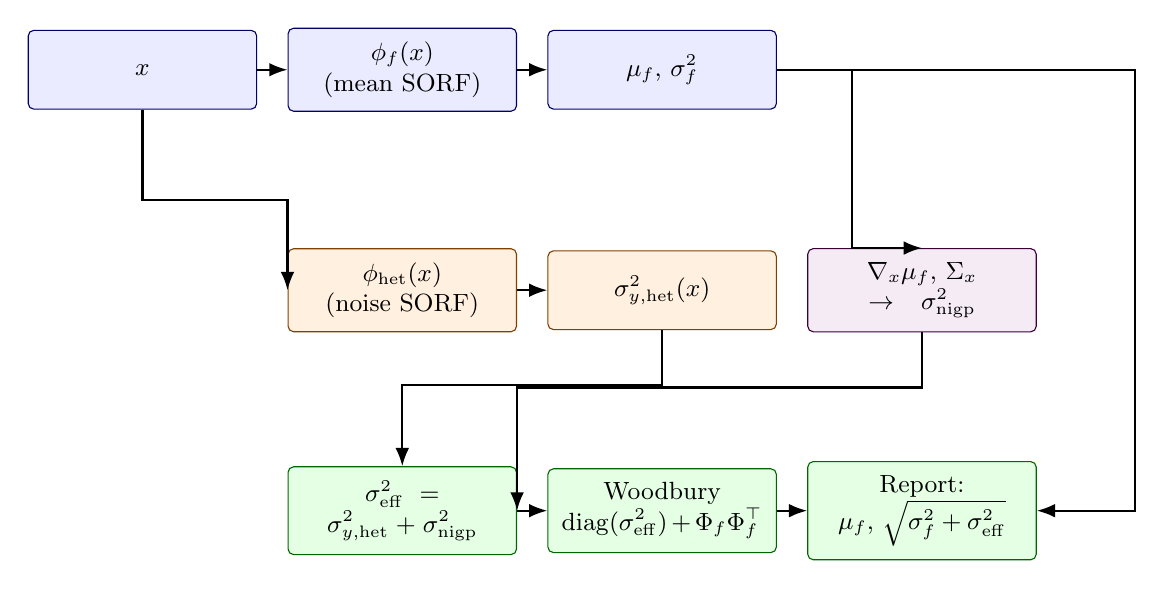
\begin{tikzpicture}[
  font=\small,
  box/.style={draw, rounded corners=2pt, align=center, inner sep=5pt,
              text width=2.55cm, minimum height=1.0cm},
  mean/.style={box, fill=blue!8, draw=blue!40!black},
  nigp/.style={box, fill=violet!8, draw=violet!45!black},
  noise/.style={box, fill=orange!12, draw=orange!50!black},
  mix/.style={box, fill=green!10, draw=green!40!black},
  arr/.style={-{Latex}, thick},
]
% Three clear rows; columns at 0 / 3.3 / 6.6 / 9.9
% Row 1: QoI mean path
\node[mean] (x)   at (0.0,  0.0) {$x$};
\node[mean] (phi) at (3.3,  0.0) {$\phi_f(x)$\\(mean SORF)};
\node[mean] (mf)  at (6.6,  0.0) {$\mu_f$, $\sigma_f^{2}$};

% Row 2: hetero (left/mid) and NIGP (right)
\node[noise] (phir) at (3.3, -2.8) {$\phi_{\mathrm{het}}(x)$\\(noise SORF)};
\node[noise] (rx)   at (6.6, -2.8) {$\sighet(x)$};
\node[nigp]  (nigp) at (9.9, -2.8) {$\gradmuf$, $\Sigx$\\$\to\;\signigp$};

% Row 3: combine → Woodbury → report
\node[mix] (d)   at (3.3, -5.6) {$\sigeff=\sighet+\signigp$};
\node[mix] (w)   at (6.6, -5.6) {Woodbury\\$\mathrm{diag}(\sigeff)+\Phif\Phif^{\top}$};
\node[mix] (out) at (9.9, -5.6) {Report:\\$\mu_f$, $\sqrt{\sigma_f^{2}+\sigeff}$};

% --- arrows (orthogonal; no box crossings) ---
\draw[arr] (x) -- (phi);
\draw[arr] (phi) -- (mf);

% x → noise SORF along the left rail
\draw[arr] (x.south) -- ++(0,-1.15) -| (phir.west);
\draw[arr] (phir) -- (rx);

% mean path → NIGP: exit right of μ_f, then down into σ_nigp (misses σ_het)
\draw[arr] (mf.east) -- ++(0.95,0) |- (nigp.north);

% σ_het and σ_nigp → σ_eff in the gap between row 2 and row 3
\draw[arr] (rx.south) -- ++(0,-0.7) -| (d.north);
\draw[arr] (nigp.south) -- ++(0,-0.7) -| (d.east);

\draw[arr] (d) -- (w);
\draw[arr] (w) -- (out);

% μ_f → report on the far-right rail (outside the NIGP/report column)
\draw[arr] (mf.east) -- ++(4.55,0) |- (out.east);
\end{tikzpicture}
\caption{Information flow for Additive Residual Hetero-NIGP with a Noise SORF
(or equivalent $\sighet$ head).
The mean SORF predicts the QoI; $\sighet$ and $\signigp$ only supply $\sigeff$.}
\label{fig:info-flow}
\end{figure}
\FloatBarrier

\section{Literature (short survey)}

\subsection{Heteroscedastic Gaussian processes}
Goldberg, Williams, and Bishop~\cite{goldberg1998heteroscedastic} place a second GP on
the log noise, so
\begin{equation}
\label{eq:goldberg}
  y\mid f,\sighet \;\sim\; \mathcal N\bigl(f,\,\sighet(x)\bigr),\qquad
  \log\sighet \;\sim\; \mathcal{GP}.
\end{equation}
Kersting et al.~\cite{kersting2007mlhgp} introduce Most Likely Heteroscedastic GP (MLHGP):
alternate between fitting the mean GP with fixed noise estimates and refitting a noise GP
to empirical squared residuals.
L\'azaro-Gredilla and Titsias~\cite{lazaro2011vhgp} give a variational treatment (VHGP)
that jointly approximates the posterior over mean and noise processes.
Snelson and Ghahramani~\cite{snelson2006variable} study variable noise in sparse GPs;
nonstationary / EP variants further relax stationarity of the noise field
\cite{tolvanen2014nonstationary,heinonen2016nonstationary}.

\subsection{Uncertain / noisy inputs}
Beyond NIGP~\cite{mchutchon2011nigp}, Girard et al.~\cite{girard2003uncertain} and
Qui\~nonero-Candela et al.~\cite{quinonero2003propagation} propagate input uncertainty
through GP predictive moments; Dallaire et al.~\cite{dallaire2009uncertain} learn under
uncertain training inputs.
These methods address \emph{input} uncertainty; they do not replace a free output-noise field
$\sighet(x)$.

\subsection{Scalable features and multitask}
Our production path uses RFF/SORF and Woodbury~\cite{rahimi2007rff,yu2016orf,cutajar2017dgp};
SVGP~\cite{hensman2013svgp} and multitask ICM~\cite{bonilla2008mtgp} are available baselines
in SpectralGPPlus.
Any free-noise model must remain compatible with diagonal-noise Woodbury (already used by NIGP).

\section{Heteroscedastic Gaussian likelihood}
\label{sec:hetero-lik}

Write a free input-dependent output variance $\sighet(x)>0$ and
\begin{equation}
\label{eq:hetero-lik}
  p(y\mid f,x)
  \;=\;
  \mathcal N\bigl(y;\,f(x),\,\sighet(x)\bigr).
\end{equation}
With RFF features the training covariance is again Woodbury-friendly:
\begin{equation}
\label{eq:hetero-woodbury}
  \Cy
  \;=\;
  \mathrm{diag}\bigl(\sighet(x_1),\ldots,\sighet(x_n)\bigr)
  +
  \Phif\Phif^{\top}.
\end{equation}
Practical parameterizations of $\ell_{\mathrm{het}}=\log_{10}\sighet$ (in increasing flexibility):
\begin{enumerate}[leftmargin=1.2em,itemsep=0.2em]
  \item \textbf{Constant} --- recovers~\eqref{eq:homo} ($\sighet\equiv\sigy$).
  \item \textbf{Parametric / small MLP} --- cheap SoftClamp on $\ell_{\mathrm{het}}(x)$.
  \item \textbf{Small second SORF} --- $D_{\mathrm{het}}\ll D_f$ features for $\ell_{\mathrm{het}}$;
        keep mean features large.
  \item \textbf{Full noise GP} --- Goldberg / MLHGP / VHGP
        \cite{goldberg1998heteroscedastic,kersting2007mlhgp,lazaro2011vhgp}; heaviest.
\end{enumerate}
For S4 we recommend starting at (2) or (3): they reuse the existing
$\mathrm{diag}(\sigeff)$ MLL path without a second $O(n^3)$ GP.

\section{Why this data wants free heteroscedasticity}

S4 independent QoI models use $X\in\mathbb{R}^{n\times 287}$ (285-band EMIT TOA radiance
plus $\cos\mathrm{zen}$ and elevation) to predict
$\{\texttt{cos\_i},\texttt{grain\_size},\texttt{dust},\texttt{algae},\texttt{cwv},\texttt{lwc},\texttt{aot}\}$
\cite{thompson2020emit,Bohn03172025}.
Noise sources are not exchangeable:

\begin{center}
\small
\begin{tabularx}{\textwidth}{@{}>{\raggedright\arraybackslash}p{0.30\textwidth}
  >{\raggedright\arraybackslash}p{0.32\textwidth}
  >{\raggedright\arraybackslash}X@{}}
\toprule
\textbf{Source} & \textbf{Natural model} & \textbf{Comment} \\
\midrule
Instrument / band SNR, scaling, registration
& NIGP $\Sigx$ / $\sigma_{x,k}^{2}$ (optionally NEDL-informed)
& Input uncertainty; ISOFIT-style OE context~\cite{thompson2018isofit} \\[0.4em]
RT / forward-model misspecification, sim--reality gap, QoI-dependent residual structure
& Free $\sighet(x)$
& Varies with scene; not a pure $\gradmuf$ effect \\
\bottomrule
\end{tabularx}
\end{center}

\vspace{0.75em}
Using only NIGP forces all nonstationarity of residuals into $\Sigx$ and slopes.
Using only free $\sighet$ ignores physically motivated input noise on radiance.
The combination below assigns each term a distinct job.

\begin{figure}[t]
\centering
\begin{tikzpicture}[
  font=\small,
  node distance=1.15cm and 1.35cm,
  box/.style={draw, rounded corners=2pt, align=center, inner sep=6pt,
              text width=2.9cm, minimum height=1.15cm},
  in/.style={box, fill=blue!8, draw=blue!40!black},
  out/.style={box, fill=orange!12, draw=orange!50!black},
  mix/.style={box, fill=green!10, draw=green!40!black},
  arr/.style={-{Latex}, thick},
]
\node[in] (nedl) {Instrument NEDL / band SNR};
\node[in, right=of nedl] (sigx) {$\Sigx$ / $\sigma_{x,k}^{2}$};
\node[out, below=1.45cm of nedl] (rt) {RT misspec.\ /\ QoI residual};
\node[out, right=of rt] (rx) {$\sighet(x)$};
\node[mix, below=1.45cm of sigx] (d) {$\sigeff=\sighet+\signigp$};
\node[mix, below=1.25cm of d] (w) {Woodbury $\mathrm{diag}(\sigeff)+\Phif\Phif^{\top}$};
\draw[arr] (nedl) -- (sigx);
\draw[arr] (rt) -- (rx);
\draw[arr] (sigx) -- (d);
\draw[arr] (rx) -- (d);
\draw[arr] (d) -- (w);
\node[font=\footnotesize\itshape, text=gray!60!black, left=0.15cm of d]
  {$\gradmuf$ from frozen dual};
\end{tikzpicture}
\caption{Scientific noise split for Additive Residual Hetero-NIGP:
input uncertainty through $\sigma_{x,k}^{2}$, residual output heteroscedasticity through
$\sighet(x)$, combined as $\sigeff$ for Woodbury.}
\label{fig:noise-split}
\end{figure}
\FloatBarrier

\section{Combining NIGP with heteroscedastic output noise}

\subsection{Primary recommendation: Additive Residual Hetero-NIGP}
\label{sec:additive}

Replace the scalar $\sigy$ in~\eqref{eq:nigp-d} by a free field $\sighet(x)$:
\begin{equation}
\label{eq:additive}
  \sigeff(x_i)
  \;=\;
  \underbrace{\sighet(x_i)}_{\text{free hetero output}}
  +
  \underbrace{\signigp(x_i)}_{\text{NIGP input propagation}}.
\end{equation}
Keep the McHutchon two-step structure: compute $\gradmuf$ from a dual solve that
treats output noise as frozen (homoskedastic $\sigy$ or frozen $\sighet$), detach the Jacobian,
then form~\eqref{eq:additive} for the MLL / predictive intervals.
This is a one-line generalization of SpectralGPPlus
\texttt{effective\_noise\_variance}: allow \texttt{noise\_y} of shape $(n,)$ instead of a scalar.

\paragraph{Asymmetric train / test (extends current practice).}
Train MLL with train-side $\sigeff(x_i)$ from~\eqref{eq:additive}.
At test, evaluate $\sighet(x_*)$ and test-side $\gradmuf(x_*)$ separately for observation
intervals (NIS / coverage), matching the existing train-$\sigeff$ / test-$\gradmuf$ split used by NI-SORF.

\subsection{Additional combination ideas}
\label{sec:ideas}

\begin{enumerate}[leftmargin=1.2em,itemsep=0.45em]
  \item \textbf{Instrument-anchored $\Sigx$, free $\sighet(x)$.}
  Fix or strongly prior $\sigma_{x,k}^{2}$ from EMIT NEDL (in scaled $x$-space); learn only residual
  hetero. Improves identifiability when both terms could explain the same residuals.

  \item \textbf{Phased unlock schedule (S5).}
  Hom: $\sigma_{y,\mathrm{hom}}^{2}$;
  NIGP: unlock $\Sigx$ with Noise SORF still frozen;
  Het refine: unlock Noise SORF $\sighet(x)$ on top of $\signigp$
  (\texttt{HeteroNIGPScheduleCallback}; see~\S\ref{sec:s5-schedule}).
  Slope refresh of $\signigp$ at NIGP unlock and at the last epoch only.

  \item \textbf{Multiplicative SNR coupling.}
  \[
    \sigeff(x_i)
    \;=\;
    \sighet(x_i)\,
    \bigl(1+\alpha\,\signigp(x_i)\bigr).
  \]
  Models scenes where larger input-propagated uncertainty also inflates residual scale.

  \item \textbf{Shared latent log-noise.}
  One latent $\ell_{\mathrm{het}}(x)$ drives $\sighet=10^{\ell_{\mathrm{het}}}$ and scales a subset of atmospheric
  $\sigma_{x,k}^{2}$, encoding that the same conditions hurt input SNR and retrieval residual.

  \item \textbf{QoI-coupled multitask noise.}
  On the MTGP path~\cite{bonilla2008mtgp}, place an ICM-style coregionalization on
  $\ell_{\mathrm{het},t}(x)$ so related QoIs share heteroscedastic structure while means remain joint
  or independent.

  \item \textbf{SORF-for-noise.}
  Use a small SORF map ($D_{\mathrm{het}}\ll D_f$) for $\ell_{\mathrm{het}}(x)$; keep mean features large.
  Stabilizes learning relative to a full second exact noise GP
  \cite{goldberg1998heteroscedastic,lazaro2011vhgp}.
\end{enumerate}

\section{Identifiability and training}

Without structure, $\sighet(x)$ and $\signigp(x)$ are partially confounded: both inflate
diagonal entries of $\Cy$.
Mitigations we recommend documenting in experiments:

\begin{itemize}[leftmargin=1.2em,itemsep=0.25em]
  \item Scientific priors: instrument-informed $\Sigx$; free $\sighet$ for residual only
        (idea~1 above).
  \item Phased unlock (idea~2): matches McHutchon's alternate optimize / refresh-slope scheme
        \cite{mchutchon2011nigp} and current SpectralGPPlus freeze windows.
  \item SoftClamp on $\ell_{\mathrm{het}}=\log_{10}\sighet$ analogous to existing noise bounds
        (e.g.\ floor near $10^{-5}$).
  \item Optional warm-start of $\sighet(x)$ from ASD scene stds / neighbor residual maps
        (validation-informed prior; not required for v1).
  \item Per-QoI independent $\sighet,t$ first (matches S4); multitask noise later (idea~5).
\end{itemize}

\section{Experiment sketch (follow-on)}

On S4 ($\sim$10k train / 25k test, 7 independent QoIs), compare per QoI:

\begin{center}
\small
\begin{tabular}{@{}llll@{}}
\toprule
\textbf{ID} & \textbf{Model} & $\Sigx$ / $\sigma_{x,k}^{2}$ & $\sighet(x)$ \\
\midrule
H0 & Homoscedastic SORF & off & $\equiv\sigy$ (constant) \\
H1 & NIGP-only (current) & learn & $\equiv\sigy$ (constant) \\
H2 & Hetero-only & off & free \\
H3 & Additive Residual Hetero-NIGP & learn & free \\
\bottomrule
\end{tabular}
\end{center}

\vspace{0.75em}
\textbf{Metrics:} RRMSE (point accuracy); NIS analogues and ASD interval coverage
(calibration); wall-clock train / predict.
\textbf{Success:} H3 improves calibration vs H1 without hurting RRMSE; H2 vs H3 and
H1 vs H3 show that $\sighet$ and $\signigp$ are not redundant.

\section*{Code pointers (SpectralGPPlus)}

\begin{itemize}[leftmargin=1.2em,itemsep=0.2em]
  \item Homoscedastic likelihood:
        \texttt{gpplus/likelihoods/log\_gaussian\_likelihood.py}
  \item NIGP $\sigeff$ and dual weights:
        \texttt{gpplus/utils/nigp\_utils.py}
        (\texttt{effective\_noise\_variance}; per-point $\sighet$ supported)
  \item Noise SORF + additive combine:
        \texttt{gpplus/utils/hetero\_noise.py}
  \item Diag-noise Woodbury:
        \texttt{gpplus/utils/rff\_utils.py};
        MLL: \texttt{gpplus/training/nigp\_mll.py}
  \item Freeze / S5 schedule:
        \texttt{gpplus/training/callbacks.py}
        (\texttt{NIGPInputNoiseFreezeCallback}, \texttt{HeteroNIGPScheduleCallback})
  \item S4 entry:
        \texttt{experiments\_SORF/S4\_emit\_SORF.py},
        \texttt{emit\_s4\_sorf\_base.py}
  \item S5 entry:
        \texttt{experiments\_SORF/S5\_emit\_heteroscedastic\_SORF.py}
\end{itemize}

\paragraph{S5 v1 implemented.}
Per-point $\sighet$ from Noise SORF MAP mean; additive $\sigeff=\sighet+\signigp$;
three-phase schedule with endpoint $\signigp$ refreshes
(see~\S\ref{sec:s5-schedule}).

\section*{One-sentence talk line}

``NIGP explains input-driven effective noise $\signigp$; a free heteroscedastic
$\sighet(x)$ explains the residual scene-dependent output noise that slopes cannot---add
them as $\sigeff=\sighet+\signigp$ on the diagonal and keep the same Woodbury path.''

\bibliographystyle{unsrtnat}
\bibliography{ref}

\end{document}
